\documentclass[letterpaper]{article} % DO NOT CHANGE THIS
\usepackage{aaai2027}  % DO NOT CHANGE THIS (fonts are loaded by the style: newtxtext, helvet, courier)
\usepackage[hyphens]{url}  % DO NOT CHANGE THIS
\usepackage{graphicx} % DO NOT CHANGE THIS
\urlstyle{rm} % DO NOT CHANGE THIS
\def\UrlFont{\rm}  % DO NOT CHANGE THIS
\usepackage{natbib}  % DO NOT CHANGE THIS AND DO NOT ADD ANY OPTIONS TO IT
\usepackage{caption} % DO NOT CHANGE THIS AND DO NOT ADD ANY OPTIONS TO IT
\frenchspacing  % DO NOT CHANGE THIS

% --- Packages added for this paper ---
\usepackage{amsmath,amssymb}
\usepackage{booktabs}
\usepackage{array}
\usepackage{colortbl}
\usepackage{xcolor}
\usepackage[ruled,vlined,linesnumbered]{algorithm2e}
\usepackage{tikz}
\usetikzlibrary{arrows.meta,positioning,fit,backgrounds,calc,shapes.misc}
\usepackage{newfloat}
\usepackage{listings}
\usepackage{fancyhdr}
\DeclareCaptionStyle{ruled}{labelfont=normalfont,labelsep=colon,strut=off}
\lstset{basicstyle={\scriptsize\ttfamily},aboveskip=2pt,belowskip=0pt,showstringspaces=false,
        breaklines=true,columns=fullflexible,keepspaces=true}

% Unified aesthetic color palette
\definecolor{ours}{HTML}{C2410C}      % Deep Terracotta / Rust: SARBLOH
\definecolor{base}{HTML}{2563EB}      % Slate Blue: Duck Baseline
\definecolor{ink}{HTML}{0F172A}       % Slate 900: Primary Text
\definecolor{muted}{HTML}{64748B}     % Slate 500: Neutral Muted
\definecolor{paper}{HTML}{FAF7F0}     % Alabaster Paper
\definecolor{oursTint}{HTML}{ECEEFF}  % table highlight for our column (pale periwinkle)
\definecolor{indigo}{HTML}{5B50E6}    % table accent: hatched indigo
\definecolor{periwinkle}{HTML}{939BFF}
\definecolor{lavender}{HTML}{A090FF}
\definecolor{gridc}{HTML}{D3D3D6}     % faint table rules
\definecolor{soft}{HTML}{FFF7ED}      % Soft Orange Tint
\definecolor{softb}{HTML}{EFF6FF}     % Soft Blue Tint

\newcommand{\code}[1]{\texttt{#1}}
\newcolumntype{L}[1]{>{\raggedright\arraybackslash}p{#1}}
\newcommand{\algcomment}[1]{\footnotesize\itshape\textcolor{muted}{#1}}
\SetCommentSty{algcomment}
\SetKwComment{Comment}{$\triangleright$\ }{}
\SetKwProg{Fn}{function}{}{end}
\SetAlFnt{\small}
\SetAlCapFnt{\small}

\pdfinfo{
/TemplateVersion (2027.2)
}

\setcounter{secnumdepth}{2}

\nocopyright  % no AAAI copyright slug on page 1; the running footer below carries the label

% Running footer: "arXiv preprint" on every page, including the title page
\fancypagestyle{plain}{%
  \fancyhf{}%
  \renewcommand{\headrulewidth}{0pt}%
  \setlength{\footskip}{20pt}%
  \fancyfoot[C]{\footnotesize\textcolor{muted}{arXiv preprint}}%
}
\pagestyle{plain}

\title{\textsc{Sarbloh}: Structured Geometric Perception and Speculative Code Execution for Autonomous ARC-AGI-3 Agents}
\author{
    Harsidak Singh Banwait
}
\affiliations{
    Independent Researcher\\
    \texttt{harsidak.singh.banwait.13@gmail.com}
}

\begin{document}

\maketitle
\thispagestyle{plain}

\begin{abstract}
Autonomous skill acquisition in uninstructed, interactive environments represents a foundational benchmark for artificial general intelligence. The ARC-AGI-3 benchmark formalizes this inductive reasoning challenge via Relative Human Action Efficiency (RHAE), penalizing superfluous exploratory actions quadratically under severe resource bounds: strictly offline execution, a single consumer-grade enterprise GPU, and a hard nine-hour wall-clock limit. While frontier reasoning models exhibit strong symbolic deduction when provided with high-level declarative state descriptions, we demonstrate that spatial grounding and visual abstraction---not policy deduction---constitute the primary operational bottleneck. When exposed to raw, unparsed $64{\times}64$ integer matrices, frontier models squander hundreds of exploratory actions deducing elementary mechanics that human players grasp within milliseconds, exhausting their action budgets before formulating coherent plans. We introduce \textsc{Sarbloh}, an end-to-end autonomous agent engineered around a high-throughput, deterministic host-side perception engine and a speculative code-as-action execution runtime. The perception engine decomposes each environment frame in $\mathcal{O}(HW)$ time ($\approx$35\,ms) into three structurally aligned representations: an object-centric symbolic state with bipartite identity tracking across temporal steps, an explicit geometric briefing that isolates mathematically verifiable spatial invariants (reachability lattices, spatial enclosures, midpoint tethers, and dihedral symmetries under $D_4 \times \mathbb{Z}^+$) from affordance hypotheses paired with unit verification actions, and an affordance-annotated spatial map. Operating over these representations, \textsc{Sarbloh} employs an embedded Python execution kernel to synthesize executable world models and multi-step action trajectories, combined with an append-only KV-cache management architecture that maintains a 98.4\% prefix-cache reuse rate on a 125B hybrid Mixture-of-Experts backbone, and a utility-driven priority scheduler that dynamically multiplexes GPU compute across 25 concurrent environments. In controlled visual comprehension rubrics, our structured perception engine improves affordance identification from 3/28 to 25/28 compared to conventional tokenized encodings while reducing input token consumption by 89.4\%. Evaluated on a single NVIDIA RTX PRO 6000 GPU across all 25 public ARC-AGI-3 environments, \textsc{Sarbloh} resolves 143 of 183 levels in 8.2 hours, discovering distinct solutions substantially earlier than the Milestone~\#1 winning baseline. On the official hidden Kaggle evaluation suite, \textsc{Sarbloh} achieved a verified efficiency score of 16.53---a 13.7$\times$ improvement over the milestone baseline. All code, model serving scripts, and verification artifacts are released under the Apache-2.0 license.
\end{abstract}

\vspace{0.4em}
\noindent\textbf{Code:} \url{https://github.com/Harsidak/SARBLOH}
\vspace{0.6em}

% Headline empirical teaser figure placed after abstract (BAPO-style empirical teaser)
\begin{figure*}[t]
\centering
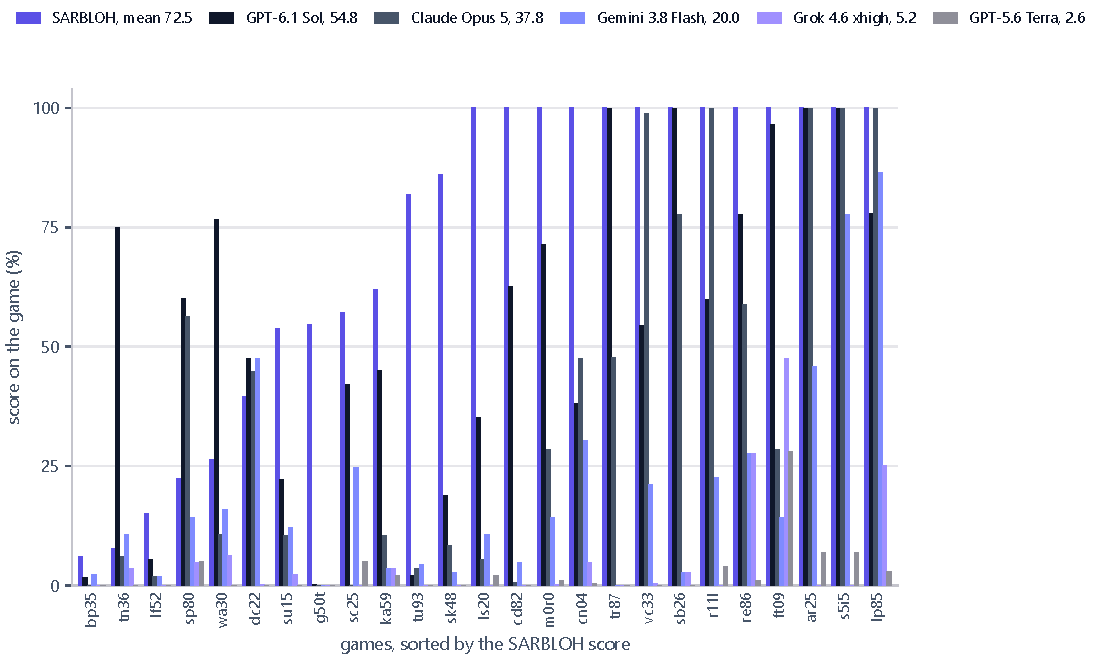
\includegraphics[width=\textwidth]{figures/per_game.pdf}
\caption{Score on the 25 public ARC-AGI-3 games. One group of bars per game, sorted by the \textsc{Sarbloh} score: the first (indigo) bar is \textsc{Sarbloh} with an open-weight Qwen3.8-Flash-Next model on one GPU, the other five are frontier models. The mean over the 25 games is 72.5 for \textsc{Sarbloh}, 54.8 for GPT-6.1 Sol, 37.8 for Claude Opus 5, 20.0 for Gemini 3.8 Flash, 5.2 for Grok 4.6 xhigh and 2.6 for GPT-5.6 Terra. \textsc{Sarbloh} reaches 100\% on 13 games. These are public-game scores, which are not comparable to the hidden-set score in Table~\ref{tab:field}.}
\label{fig:pergame}
\end{figure*}

\section{Introduction}
\label{sec:intro}

This is the introduction. Introduce the context and motivate your work here.
You can cite a paper like this: \cite{smith2023example}.

\section{Preliminaries}
\label{sec:prelim}

\subsection{ARC-AGI-3 and its score}
An ARC-AGI-3 environment is a turn-based game made of a sequence of levels \citep{arcagi3}. At each step the agent
receives a frame, a grid of up to $64{\times}64$ cells with one of 16 colours each, together with the game state
(\code{NOT\_FINISHED}, \code{WIN}, \code{GAME\_OVER}) and the number of levels completed so far. It answers with one
action: \code{ACTION1}--\code{ACTION4} (directions), \code{ACTION5} (a game-specific key), \code{ACTION6}$(x,y)$ (a
click), \code{ACTION7}, or \code{RESET}. Nothing tells the agent what any action does, what it controls, or what
counts as winning. Early levels teach a mechanic and later levels compose several. The games use only core-knowledge
priors \citep{spelke2007core}: objects, agents, goals, number and elementary geometry.

The score is \emph{Relative Human Action Efficiency} (RHAE). Let $h_{l}$ be the human baseline for level $l$ (the
upper-median best human action count) and $a_{l}$ the agent's action count. Then
\begin{equation}
S_l = \min\!\Big(1.15,\, \big(\tfrac{h_l}{a_l}\big)^2\Big),\quad
E = \frac{\min\!\big(\sum_{l\le k} l,\; \sum_{l\le n} l\, S_l\big)}{\sum_{l\le n} l},
\label{eq:rhae}
\end{equation}
where $k$ of the $n$ levels were completed, and the benchmark score is the mean of $E$ over games. Three properties
drive everything that follows. Reasoning is free and only committed actions count. The penalty is \emph{quadratic},
so an agent that needs twice the human's actions keeps a quarter of the credit. Later levels weigh more, so the
mechanics learned early pay off late.

\subsection{The offline Kaggle setting}
The Kaggle track reruns a submitted notebook on hidden games, without internet access. Our measured hardware is one NVIDIA RTX PRO 6000
Blackwell (96\,GB), 176\,GB of RAM and a nine-hour limit on the GPU notebook. Every model must be open-weight and loaded
from an attached dataset. In practice the budget is fixed in GPU-hours, so what an agent can afford to think is
limited by tokens per second, and what it can afford to see is limited by the prompt length the cache keeps warm.

\subsection{How ARC has been attacked}
\paragraph{Static ARC.} The first ARC competitions were won by search over hand-written domain-specific languages
\citep{wind2020icecuber}. Later work added object graphs \citep{xu2023arga}, library learning \citep{ellis2021dreamcoder}
and minimum-description-length pressure \citep{ferre2025madil}. The ARC Prize 2024 winners moved to neural methods:
test-time training \citep{akyurek2024ttt,arcprize2024}, combined induction and transduction \citep{li2024induction},
and later tiny recursive networks \citep{jolicoeur2025trm}. These systems map a few input--output pairs to one answer.
They never have to act.

\paragraph{Agents for ARC-AGI-3.} Interactive ARC rewards a different design. General LLM agents interleave reasoning
and acting \citep{yao2022react} or grow a library of code skills \citep{wang2023voyager}. Symbolica's \emph{Arcgentica}
\citep{knutsen2026arcgentica} uses an orchestrator that never touches the game and delegates to subagents that return
compressed summaries, which keeps the context small. \emph{VISTA} \citep{vista2026} is a visual harness with lossless
frame memory. \emph{Executable World Models} \citep{rodionov2026ewm} keep a Python model of the game, verify it
against every past step, and plan through it, in the spirit of WorldCoder \citep{tang2024worldcoder} and code world
models \citep{lehrach2025cwm}. \emph{Tycho} \citep{lehmann2026tycho} induces programmatic world models. Graph-based
exploration \citep{rudakov2025graph} needs no training and ranks actions by salience. \emph{Prime Agent}
\citep{karten2026prime} gives a frontier model one persistent IPython REPL and reports a large ARC-AGI-3 gain from the
harness alone; our harness started as a port of its host loop. All of these use frontier API models. Their numbers come
from the 25 public games, which are partly memorised by now, and none of them runs offline.

\paragraph{The open-weight field.} The comparison class for this paper is the Kaggle offline track
(Table~\ref{tab:field}). Milestone~\#1 (June 2026) was won by Tufa Labs' \emph{Duck} \citep{duck2026,arcprizemilestone1}.
It runs Qwen~3.6 27B locally inside a Python REPL that exposes the game as variables, perceives through images, ASCII
grids and segmentation, and evicts its oldest messages so it can play indefinitely. Its authors found that hand-crafted
tools hurt and that letting the model improvise worked better. Second and third place both ran Gemma-4-31B as a
vision model that emits JSON actions from labelled frames \citep{arcprizemilestone1}.

\begin{table}[t]
\centering
\small
\setlength{\tabcolsep}{3.5pt}
\begin{tabular}{@{}llcr@{}}
\toprule
System & Model & Offline & Score \\
\midrule
\multicolumn{4}{@{}l}{\emph{Public games, frontier APIs (self-reported)}} \\
Exec.\ World Models & GPT-5.5 & -- & 58.1 \\
Prime Agent & frontier & -- & 95.5 \\
Arcgentica, VISTA, Tycho & frontier & -- & high \\
\midrule
\multicolumn{4}{@{}l}{\emph{Hidden games, Kaggle, one GPU}} \\
Reki (M\#1, 2nd) & Gemma-4-31B & \checkmark & 0.87 \\
Duck (M\#1, 1st) & Qwen 3.6 27B & \checkmark & 1.21 \\
\textbf{\textsc{Sarbloh} (ours)} & \textbf{Flash-Next} & \checkmark & \textbf{16.53} \\
\bottomrule
\end{tabular}
\caption{Where \textsc{Sarbloh} sits. The two halves are not comparable: one is the public set with unbounded
frontier inference, the other the hidden set on one GPU. M\#1 scores are from June. The leaderboard has moved since
(\S\ref{sec:results}).}
\label{tab:field}
\end{table}

\section{Motivation: Isolating the Visual Grounding Bottleneck}
\label{sec:motivation}

Prior to constructing our agent architecture, we conducted a sequence of controlled ablation experiments designed to isolate the exact computational failure modes where autonomous language model agents squander their action budgets in interactive reasoning tasks.

\paragraph{The Representation Ladder.}
We evaluated a state-of-the-art frontier model (Gemini 1.5 Pro) on the inaugural level of \code{ls20}---a representative ARC-AGI-3 environment featuring a discrete keyboard-navigated maze with directional barriers, an inventory key, a locking mechanism, and a dynamic action gauge. Holding the model, prompt instructions, and underlying environment strictly constant, we systematically modulated only the modality and structure of the input observation (Figure~\ref{fig:gemini}).

\begin{figure}[t]
\centering
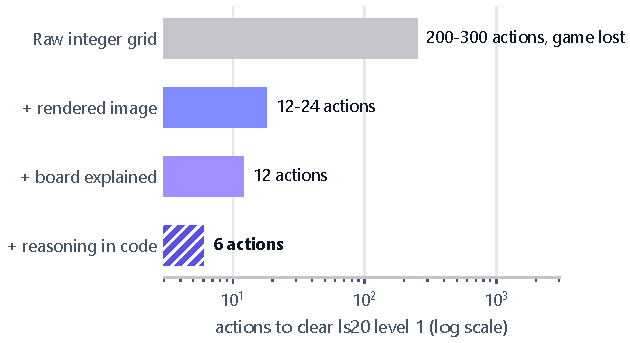
\includegraphics[width=\columnwidth]{figures/gemini_ladder.pdf}
\caption{Controlled ablation of input observation modalities on the first level of \code{ls20}, evaluated using an identical frontier reasoning model. Serializing the environment as raw integer tokens induces catastrophic exploration failure (200--300 actions, exceeding budget). Providing a rendered visual frame reduces required actions by over an order of magnitude (14$\times$ speedup), while augmenting the state with deterministic geometric relations and programmatic execution achieves super-human efficiency (6 actions versus human baseline $\approx$10).}
\label{fig:gemini}
\end{figure}

When provided solely with the raw $64{\times}64$ integer matrix and the valid action enumeration, the model expended between 200 and 300 exploratory actions, repeatedly colliding with invisible topological boundaries and ultimately exhausting the action budget without reaching the goal state. Serializing spatial lattices into discrete token sequences destroys spatial adjacency priors: evaluating topological reachability across 4,096 integer tokens requires quadratic attention across distant positions in the sequence, an operation that autoregressive attention heads fail to execute reliably \citep{rahmanzadehgervi2024blind}. 

Conversely, supplying the identical model with a rendered 2D image of the identical board immediately reduced action expenditure to 12--24 actions---an operational speedup exceeding an order of magnitude achieved purely by aligning the state representation with visual pre-training priors. Augmenting the visual frame with a structural decomposition of board components (delineating static terrain, dynamic gauges, and color parity invariants) further condensed the trajectory to 12 actions. Finally, prompting the model to synthesize programmatic search scripts within an execution sandbox yielded optimal completion in exactly 6 actions. The primary performance leap stems from perceptual grounding rather than scale of reasoning.

\paragraph{The Oracle Briefing: Decoupling Perception from Planning.}
To determine whether agent failures originate from deficiencies in high-level policy planning or low-level perceptual parsing, we performed an oracle comprehension experiment. The model was tasked with solving an advanced level of \code{ls20} under two conditions: (i) providing visual screenshots alone, and (ii) augmenting visual screenshots with an ``oracle briefing''---a concise, structured natural language annotation specifying inferred action semantics, goal criteria, mechanical dependencies, and identified on-screen entities.

Without the briefing, the agent squandered its entire action allocation exploring inert visual artifacts and failed to resolve the level. In the presence of the structural briefing, the model formulated an optimal plan and cleared the level in 6 actions, substantially outperforming the author's initial blind playthrough ($\approx$10 actions). This empirical divergence establishes a vital architectural insight: modern reasoning backbones possess highly capable sequential planning and programmatic search capabilities, but their execution remains bottlenecked by inaccurate visual state induction. If an agent can be provided with high-fidelity semantic and geometric grounding, its downstream planning executes with near-optimal efficiency.

\paragraph{The Failure of Sparse Coordinate Deltas.}
In resource-constrained settings, a common optimization is transmitting only sparse coordinate deltas (i.e., the set of grid cells modified between step $t-1$ and $t$) to minimize prompt token consumption. While computationally economical, our empirical tracking revealed that coordinate deltas induce severe perceptual myopia. In ARC-AGI-3 environments, local agent actions routinely trigger non-local, global state transitions: for example, stepping onto a localized trigger tile in \code{ls20} instantaneously alters an icon situated in a distant status panel. When an agent receives only localized coordinate updates, it systematically overlooks global mechanical coupling, hallucinating that its action produced no operational side-effects. Maintaining holistic whole-frame visual representations is therefore mandatory to preserve causal tracking across the entire visual field.

\paragraph{Core Design Principles of the Perception Engine.}
Because oracle briefings cannot exist for undisclosed, held-out environments during official evaluation, an autonomous agent must construct its own structural abstractions dynamically. ARC-AGI-3 environments are strictly grounded in human core knowledge \citep{spelke2007core}, which is predominantly geometric and topological: connectivity, spatial enclosure, lattice-constrained reachability, structural symmetry, and affine transformations. 

These properties admit exact, deterministic algorithmic verification. In contrast, operational semantics (e.g., identifying which dynamic component represents the agent embodiment, or what constitutes the terminal win condition) are fundamentally latent under partial observability and can only be induced through empirical interaction. 

These findings dictate the central architectural axiom governing \textsc{Sarbloh}:
\begin{quote}
\itshape
Compute mathematically certain geometric invariants deterministically via zero-parameter host code; formulate ambiguous operational roles as explicit probabilistic hypotheses; and equip every hypothesis with a minimal-cost, single-action falsification test.
\end{quote}
By enforcing this strict dichotomy, the agent eliminates visual hallucination over spatial facts, while ensuring that any incorrect operational hypothesis is refuted through a single probing action, entirely averting catastrophic quadratic exploration penalties.
\section{Methodology}
\label{sec:method}

Perception is the part of \textsc{Sarbloh} that we developed most deliberately, so most of this section is about it: where it started (Section~\ref{sec:origins}), the eight designs we compared in a perception lab (Section~\ref{sec:lab}), what survived a held-out check (Section~\ref{sec:holdout}), and what the final engine computes (Section~\ref{sec:perception}). The last subsection (Section~\ref{sec:agent}) shows how the engine sits inside the whole agent (Figure~\ref{fig:overview}).

\subsection{Where Perception Started}
\label{sec:origins}

The first perception module, which we call the \emph{Legacy Encoder}, pushed a new observation into the context after every transition. It had four parts: the frame as a PNG in the ARC palette ($4\times$ nearest-neighbour, $256{\times}256$ pixels); a lettered board with one letter per colour, shown whole at the start of a level and afterwards only as the changed region with a 3-cell margin and numbered rows and columns; a segmentation list of 4-connected objects with id, colour, shape hash, bounding box, containment and adjacency, with HUD bars along the frame edge flagged; and one change line per transition (``\code{obj 4 moved dx=0 dy=-5; obj 9 vanished; 2 cells recoloured}''). It cost about 3{,}500 text tokens per frame.

Three early probes on the first level of \code{ls20} shaped it. They are qualitative, were logged from the author's own runs, and have no held-out score.
\begin{itemize}
    \item \textbf{Whole-frame picture versus cell deltas.} Sending only the changed cells is cheaper, but some actions change the game globally (stepping onto the modifier in \code{ls20} does), and a cell-delta view hides that. A whole-frame picture kept the global effect visible.
    \item \textbf{Picture plus segmentation text.} The model understood the frame precisely only when the segmentation list and the lettered board came beside the picture: the picture carries the global layout, the text carries exact positions.
    \item \textbf{Oracle briefing.} A frontier model played the same level twice, once from screenshots and the action space alone and once with a briefing we wrote by hand (action meanings, goal, mechanics, on-screen components). Without the briefing the game was wasted; with it the level was cleared in about six actions, against about ten for the author. Execution was adequate and understanding was the bottleneck (the ladder of Figure~\ref{fig:gemini}, Section~\ref{sec:motivation}).
\end{itemize}
The last probe set the target: an engine that writes the briefing itself, from the frame alone, for a game it has never seen.

\subsection{The Perception Lab: Eight Ways to Read One Frame}
\label{sec:lab}

We compared eight ways of presenting the same frame against the Legacy Encoder, one Python file each. All of them share one front end (screenshot, then an exact $64{\times}64$ palette grid, then the object list), so the only thing that changes is what is computed on top of the objects and how it is shown. The two test frames are the first levels of \code{ls20} (keyboard controls) and \code{r11l} (clicks). Understanding was graded against an answer key written and checked in the engine before any presentation ran: seven items per frame (spatial boundaries, mechanical linkages, agent identity, goal, gauges and so on) at two points each, 28 points in all, plus an intuition grade from 1 to 5. The kill rule was fixed in advance: drop a presentation that scores no better than the Legacy Encoder (3/28), or whose claims are wrong on about half or more of the held-out games.

\begin{figure*}[t]
\centering
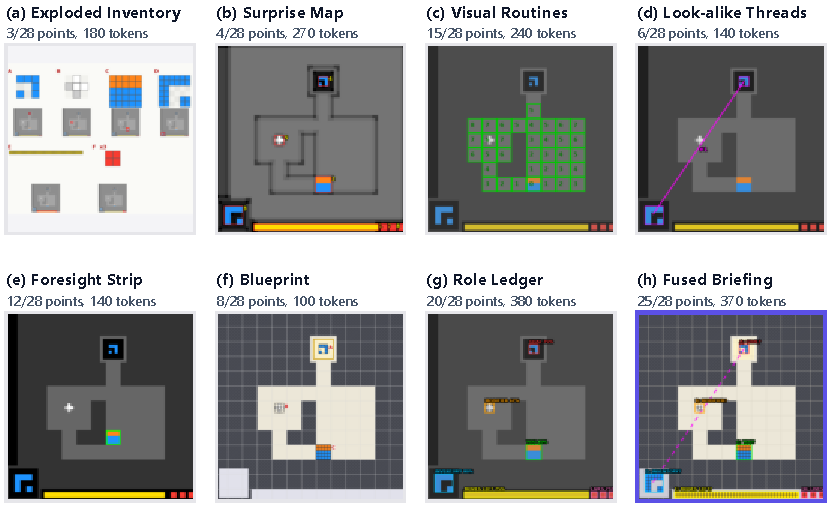
\includegraphics[width=\textwidth]{figures/perception_lab_gallery.pdf}
\caption{The image part of each candidate presentation for the opening frame of \code{ls20}, with its rubric score and its text cost per frame. (a) Exploded Inventory pulls out every object and stacks copies. (b) Surprise Map keeps colour only where the frame is unpredictable. (c) Visual Routines marks reachability, with the step count to each tile. (d) Look-alike Threads joins shapes that match under rotation, mirroring or scale. (e) Foresight Strip imagines the next frame (here, one step up). (f) Blueprint redraws floor, walls and lattice as a clean schematic. (g) Role Ledger tags each object with a guessed role and a confidence. (h) Fused Briefing, the presentation we kept, combines the blueprint with measured facts and tagged guesses.}
\label{fig:labgallery}
\end{figure*}

\begin{itemize}
    \item \textbf{Exploded Inventory} (3/28) pulls every object out of the frame, enlarges it, spaces the objects apart and stacks identical copies as $\times N$. The list is clean but attaches no meaning to anything.
    \item \textbf{Surprise Map} (4/28) ranks cells by how unpredictable their $3{\times}3$ neighbourhood is and flags broken symmetry. About 90\% of the frame is predictable texture, and the map caught the lopsided plus on \code{ls20}, but little else.
    \item \textbf{Visual Routines} (15/28), after Ullman, computes reachability by flood fill with step counts, what lies inside what, line tracing to attached objects, midpoints and alignment. On \code{r11l} it found the midpoint tether and the ring that fits a $5{\times}5$ object.
    \item \textbf{Look-alike Threads} (6/28) joins objects that are equal under rotation, flip, scale or recolouring and names the transform. On \code{ls20} it showed that the inventory icon is the goal shape turned $90^\circ$ and drawn at twice the size.
    \item \textbf{Foresight Strip} (12/28) imagines the next frame for each action from simple movement priors. On \code{ls20} it predicted all four moves and the gauge correctly, and on \code{r11l} its three-click plan solved the level.
    \item \textbf{Blueprint} (8/28) redraws the frame as a schematic: floor, walls, tile lattice, named shapes and the HUD moved to a side panel. It is the best map for navigation and says nothing about meaning.
    \item \textbf{Role Ledger} (20/28) guesses a role for every object (agent, goal, handle, gauge, lives) with a confidence and a one-action test. Every role was right on both frames.
    \item \textbf{Fused Briefing} (25/28) uses the Blueprint as its picture, states the Visual Routines and Look-alike Threads results as measured facts, and adds the Role Ledger guesses with their tests. Foresight Strip was dropped.
\end{itemize}

\begin{figure}[t]
\centering
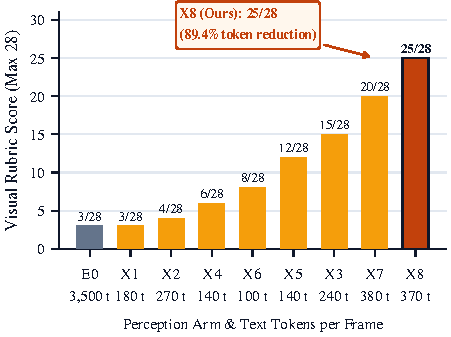
\includegraphics[width=\columnwidth]{figures/perception_lab.pdf}
\caption{Rubric score (of 28) and text tokens per frame for the Legacy Encoder and the eight presentations, on the two test frames. The Fused Briefing scores 25/28 against 3/28 for the Legacy Encoder at about a tenth of the text.}
\label{fig:lab}
\end{figure}

Exploded Inventory and Surprise Map did no better than the Legacy Encoder, at a tenth of its text, and were dropped as stand-alone presentations. What moved understanding most were the computed relations of Visual Routines and Look-alike Threads, which state facts a model cannot reliably read off a picture, and the Role Ledger, which gives the fastest gist. The Fused Briefing reached 25/28 at about 370 tokens per frame, 8.3$\times$ the Legacy Encoder's score with 89.4\% fewer text tokens. Two caveats apply. The grader was the same agent that built the presentations and knew both games, and no blind reader was used. The Fused Briefing was designed after the other eight were graded and was graded on the same two frames, so its score is optimistic.

\subsection{Held-Out Check: Facts Versus Guesses}
\label{sec:holdout}

We then checked the presentations on the 23 other official games, none of which had been used in the design. This check was graded by the engine rather than by hand (Table~\ref{tab:holdout}). Turning a screenshot into a grid generalised perfectly (23/23 games at 100\% cell accuracy). The guesses did not: they had effectively been fitted to the two test frames and were right about half the time or less on unseen games.

\begin{table}[t]
\centering
\small
\begin{tabular}{@{}L{0.55\columnwidth}L{0.36\columnwidth}@{}}
\toprule
Check on the 23 held-out games & Result \\
\midrule
Screenshot to grid, exact cells & 23/23 games \\
Agent identity, keyboard games & 6/14 games \\
Moves-left gauge found & 10/20 games \\
Click handles that respond & 7/29 handles \\
Keyboard foresight fully right & 1/16 games \\
\bottomrule
\end{tabular}
\caption{Held-out check of the single-frame guesses. For click handles, the guesses were good on \code{dc22} (2/2), \code{sb26} (4/4) and \code{ka59} (1/1) and bad on \code{lp85} (0/17). On two further keyboard games nothing moved on the first key press, so the agent-identity guess could not be checked.}
\label{tab:holdout}
\end{table}

This fixed the design rule of the engine: \emph{computed relations (reachability, enclosure, tethers and midpoints, alignment, shape equivalence) are stated as facts, because they are true by construction, whereas roles and dynamics from a single frame are stated as guesses, each with a one-action test that settles it}. One real action answers what a single-frame prior cannot. We did not run the Fused Briefing as a whole on the held-out games, and the lab reports no RHAE. The end-to-end effect of the engine on the agent is not isolated by an ablation: the trajectory of Section~\ref{sec:trajectory} changes several components at once.

\subsection{The Perception Engine}
\label{sec:perception}

The final engine is the Fused Briefing, rewritten to work directly on the grid inside the agent. It is about 1{,}500 lines of host-side NumPy and Pillow with no learned parameters. Over 225 real frames (the first frame and eight random actions on each of 25 offline games) it raised no errors, with a median of 42\,ms for the briefing and 40\,ms for the picture (maximum 0.38\,s for a briefing). For every environment transition it generates three synchronized representations sharing one persistent object identity space (Figure~\ref{fig:views}, Algorithm~\ref{alg:perceive}).

\begin{figure*}[t]
\centering
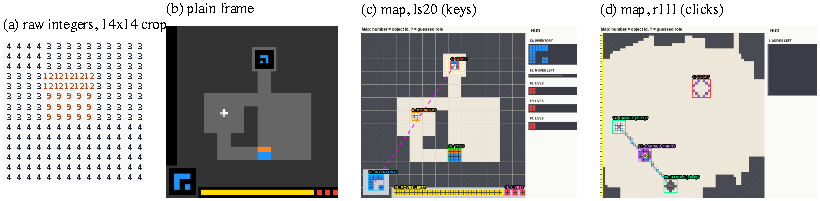
\includegraphics[width=\textwidth]{figures/perception_views.pdf}
\caption{Structural multimodal representation of an ARC-AGI-3 frame produced by the perception engine. (a) Conventional serialization provided to language models: an unparsed matrix of discrete integer tokens ($14{\times}14$ crop of a $64{\times}64$ frame). (b) Rendered 2D visual frame. (c, d) Affordance-annotated perception maps generated for the opening frames of \code{ls20} (discrete keyboard controls) and \code{r11l} (continuous spatial clicks). Traversal floor surfaces are rendered in light tones, impenetrable barriers are hatched, and peripheral HUD panels are isolated and scaled on the right. Tracked entities display persistent integer IDs alongside scored affordance roles. Magenta dashed threads indicate dihedral shape equivalence under rotation and scaling; yellow rings indicate mechanical midpoint tethers.}
\label{fig:views}
\end{figure*}

\paragraph{View 1: Morphological Segmentation, Tracking, and Change Ledgers.}
The background canvas is identified via the modal color index across the frame. All remaining 4-connected monochromatic components are segmented into discrete entities characterized by spatial bounding boxes, exact pixel masks, adjacency matrices, and topological containment hierarchies. On the initial frame of a level, entities are assigned persistent identifiers in standard raster reading order. On subsequent frames, an invariant bipartite matching algorithm tracks entity persistence across five sequential priority passes:
\begin{enumerate}
    \item \emph{Rigid Invariance}: Identical shape hash, color index, and spatial coordinates.
    \item \emph{Spatial Translation}: Identical shape hash and color index with translated coordinates.
    \item \emph{State Recoloring}: Identical shape hash and spatial coordinates with altered color index.
    \item \emph{Morphological Deformation}: Identical color index with significant spatial overlap ($>50\%$ IoU).
    \item \emph{Novel Component Instantiation}: Entities unmapped by preceding passes are instantiated with fresh unique IDs.
\end{enumerate}
Consequently, symbolic references such as \code{objects[10]} within the agent's Python kernel refer to the identical physical entity across the entire level lifetime. The spatial grid is transcribed into a lettered alphanumeric matrix with explicit row and column headers. Sequential actions append a differential change ledger formatted as: ``\code{\#12 A4(right): 6 cells altered at r10-12 c20-25; HUD altered (1 cell)}''. Environmental changes within the peripheral 3-cell screen boundary are partitioned into HUD telemetry, preventing minor status updates (e.g., action counter decrements) from obfuscating playfield invariants.

\paragraph{View 2: Layout Decomposition and Verified Geometric Invariants.}
The structural briefing decomposes the playfield into macroscopic functional layouts. Color partitions spanning $>8\%$ of total frame area are classified as terrain. The remaining visual structure is decomposed into functional primitives: linear corridors, peripheral boundary gauges, composite multi-colored assemblies (clustered via union-find over 8-connected components), panel icons, and dotted figures.

Conditioned on this layout, the engine computes seven categories of mathematically verifiable \textsc{Measured Invariants}, true by geometric construction:
\begin{itemize}
    \item \textbf{Lattice Reachability}: Breadth-first search (BFS) over detected spatial lattices computes exact traversal distances from potential agent entities to all interactive targets (e.g., ``\code{obj 6 reachable in 6 steps}''; ``\code{enclosure entry accessible at bottom face in 5 steps}'').
    \item \textbf{Topological Enclosure}: Detection of closed boundaries enclosing empty spatial cavities, mapped against entities matching those cavity dimensions.
    \item \textbf{Midpoint Tethers}: Identification of linear linkages spanning entity pairs, calculating mechanical centerpoints (e.g., ``\code{obj 25 held at midpoint of obj 16 and 36; endpoint translation forces midpoint translation}'').
    \item \textbf{Coordinate Collinearity}: Verification of shared row or column alignments between key landmarks.
    \item \textbf{Dihedral Affine Symmetries}: Identification of shape equivalence under the dihedral group $D_4 \times \mathbb{Z}^+$ (spanning reflection, 90$^\circ$ rotations, and integer scaling), identifying cross-scale functional analogues (e.g., ``\code{obj 12 is a 2$\times$ scaled reflection of goal obj 4}'').
    \item \textbf{Multiplicity Counters}: Clusters of identical morphological instances, parsed as discrete countable sets (e.g., life indicators, consumable resources).
    \item \textbf{Color Polarity Asymmetries}: Detection of morphologically symmetric entities exhibiting asymmetric chromatic distributions, marking directional orientation or active operational state.
\end{itemize}

\paragraph{Affordance Role Induction and Minimal Falsification Probes.}
Subsequent to invariant verification, non-terrain components are evaluated against eight canonical game-design affordance roles via weighted evidence scoring (Table~\ref{tab:roles}). To eliminate the risk of hallucinated mental models, the engine couples each inferred role hypothesis with an explicit, single-action falsification probe:
\begin{table}[t]
\centering
\footnotesize
\setlength{\tabcolsep}{3.5pt}
\begin{tabular}{@{}L{0.22\columnwidth}L{0.37\columnwidth}L{0.35\columnwidth}@{}}
\toprule
Affordance Role & Evidentiary Priors (Scored) & Unit Falsification Probe \\
\midrule
\textsc{Player / Agent} & Compact, multi-chromatic, unique, lattice-aligned & Issue 1 directional action: verify 1-tile translation \\
\textsc{Target Goal} & Hollow receptor, bounding enclosure, HUD shape matching & Transport matching entity into enclosure \\
\textsc{Action Gauge} & Elongated peripheral bar spanning screen margin & Issue arbitrary action: verify 1-unit reduction \\
\textsc{Life Counter} & Multiple identical glyphs in peripheral HUD & Observe count upon episode reset or hazard \\
\textsc{Inventory} & Isolated HUD glyph mirroring playfield entity & Observe glyph after interacting with modifier \\
\textsc{Modifier} & Compact symbol exhibiting chromatic asymmetry & Traverse onto entity: verify inventory mutation \\
\textsc{Actuator Handle} & Tether endpoint; chromatic toggle pair & Issue coordinate click: verify spatial jump \\
\textsc{Coupled Cargo} & Mechanically constrained between two tether handles & Translate handle: verify proportional shift \\
\bottomrule
\end{tabular}
\caption{Affordance role induction rules. Each hypothesis is presented with evidentiary confidence and an explicit single-action falsification test, ensuring erroneous hypotheses are refuted at minimal action cost.}
\label{tab:roles}
\end{table}

The natural language briefing is bounded to 30 lines by default, allocating at most one-third of that budget to role hypotheses and sharing the rest among the invariant categories so that no single kind of fact can fill it; facts touching the guessed agent and goal come first, and the remainder are counted (``\code{+N more facts}'') and stay available through \code{observe().briefing}. Complete structured briefings are provided in Appendix~\ref{app:briefings}.

\paragraph{View 3: Structured Affordance Map.}
The spatial map (Figure~\ref{fig:views}c,d) renders abstracted semantic structure rather than raw pixels: accessible terrain is rendered in pale tones, impassable walls are hatched, detected lattice grids are overlaid as fine lines, and all entities are bordered by role-colored bounding markers labeled ``\code{id: ROLE?}''. Look-alike symmetries under $D_4 \times \mathbb{Z}^+$ are joined via dashed chromatic threads, while mechanical tether linkages display midpoint concentric rings. Peripheral HUD panels are isolated and magnified on the right. Crucially, natural language annotations are excluded from image pixels and transmitted strictly as structured text, maximizing token efficiency and eliminating visual OCR errors.

\paragraph{Observation Scheduling.}
The full multimodal observation (briefing text, alphanumeric grid, and rendered map) is transmitted at level inception, following context window purges, and when the agent calls \code{observe()} after acting, at most once per state. Following intermediate actions, the agent receives an abbreviated observation: the differential change ledger, a cropped alphanumeric window centered on the modified coordinate region with a 3-cell margin, and the updated visual map, consuming fewer than 600 tokens. The complete object table is retained host-side and queried on-demand via Python kernel calls (\code{observe().objects}).

\paragraph{Hardening inside the agent.}
Two problems appeared only once the engine ran on live play. First, the test for a tile lattice flipped during play: \code{ls20} lost its $5{\times}5$ grid after one move, because the gauge in the status box added off-grid edges, and \code{ka59} lost its $3{\times}3$ grid whenever the agent touched another object. Status boxes are now left out of the test and the level's previous lattice is kept while it still fits, which removed all flips on the 225 frames. Second, ``X is directly above Y'' facts crowded out everything else: on \code{tr87} they filled 27 of the 30 briefing lines (68 facts in all, and 792 on \code{bp35}). A fixed cap also deleted facts from \code{observe().briefing}, so we kept every alignment fact, put those touching the guessed agent and goal first, and let each kind of fact take only its share of the lines shown.

\begin{algorithm}[t]
\caption{\textsc{Perceive}: Deterministic Frame-to-Modality Mapping}
\label{alg:perceive}
\KwIn{Raw grid $g_t \in \{0..15\}^{H\times W}$, persistent tracker $T$, lattice prior $\Lambda'$, legal actions $\mathcal{A}$}
\KwOut{Structured briefing $B$, tracked entities $O$, visual map $M$, differential change $\delta$}
$O \gets \textsc{MorphologicalSegmentation}(g_t)$\;
$(O, \delta) \gets T.\textsc{BipartiteMatch}(O)$ \Comment*[r]{temporal identity persistence}
$\mathcal{T} \gets \{c \in \{0..15\} : |g_t{=}c| > 0.08\,HW\}$ \Comment*[r]{terrain segmentation}
$L \gets \textsc{ExtractLayout}(g_t, \mathcal{T})$\;
\ForEach{entity $e \in L$}{
  $e.\mathit{is\_hud} \gets \textsc{IsPeripheralBoundary}(e)$\;
  $e.\mathit{id} \gets \textsc{MajorityOverlapId}(e, O)$\;
}
$e_{\text{agent}} \gets \textsc{IdentifyCandidateAgent}(L, \mathcal{A})$\;
$\Lambda \gets \textsc{DetectLattice}(L) \textbf{ or } \Lambda'$\;
$F \gets \textsc{BFSReach}(e_{\text{agent}}, \Lambda) \cup \textsc{Enclosures}(L)$\;
$F \gets F \cup \textsc{Tethers}(L) \cup \textsc{Symmetries}_{D_4\times\mathbb{Z}^+}(L)$\;
\ForEach{entity $e \in L$}{
  $\boldsymbol{\sigma}_e \gets \textsc{ScoreAffordances}(e, F, \mathcal{A})$\;
  $\hat{\rho}_e \gets \arg\max_r \boldsymbol{\sigma}_e[r], \quad p_e \gets \boldsymbol{\sigma}_e[\hat{\rho}_e] / (1 + \sum_r \boldsymbol{\sigma}_e[r])$\;
}
$B \gets \textsc{FormatInvariants}(F)$\;
$B \gets B \,\|\, \textsc{FormatHypotheses}(\hat{\boldsymbol{\rho}}, \boldsymbol{p}, \textsc{Tests}(\hat{\boldsymbol{\rho}}))$\;
$M \gets \textsc{RenderAffordanceMap}(L, \hat{\boldsymbol{\rho}}, F)$\;
\Return{$(B, O, \textsc{ToAlphanumeric}(g_t)), M, \delta$}
\end{algorithm}

\subsection{The Overall \textsc{Sarbloh} Agent}
\label{sec:agent}

\begin{figure*}[t]
\centering
\resizebox{\textwidth}{!}{%
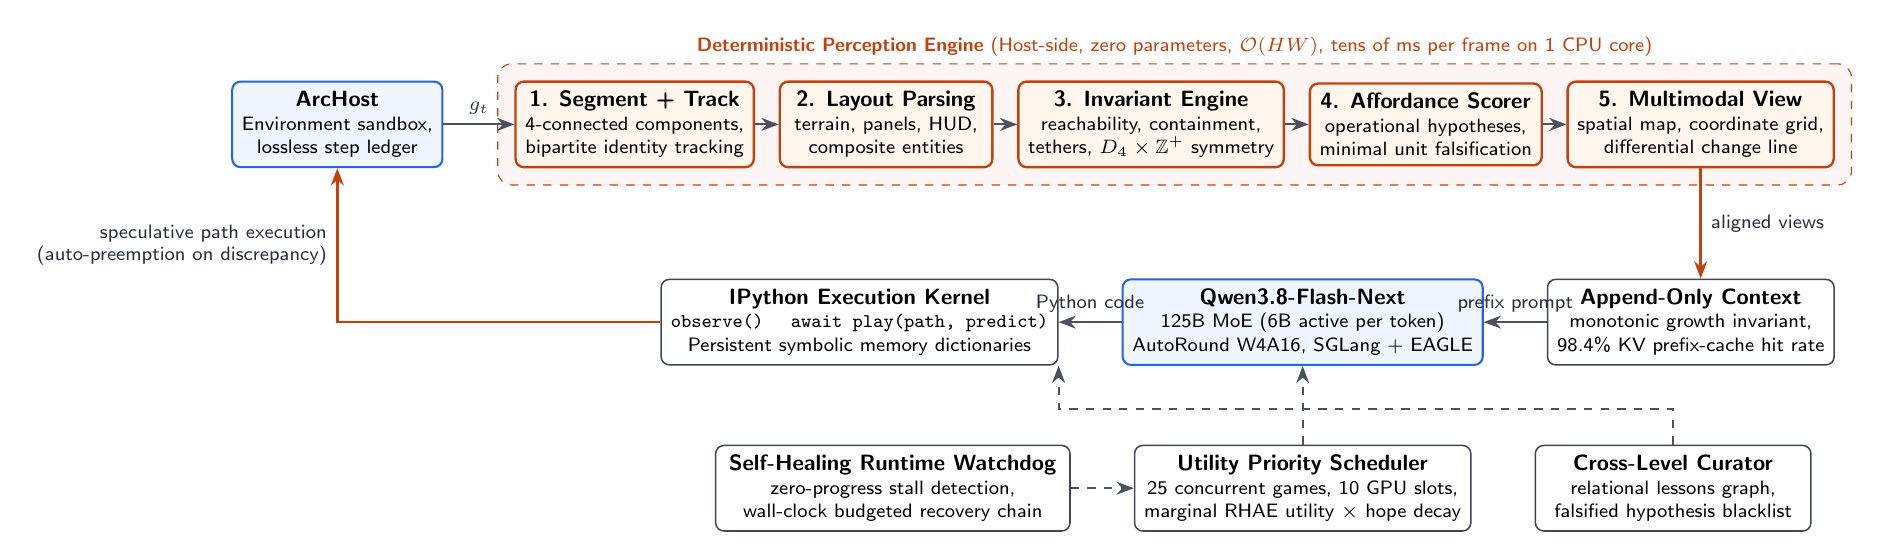
\begin{tikzpicture}[
  font=\sffamily\footnotesize, >={Stealth[length=2.2mm]},
  box/.style={draw=ink!80, rounded corners=3pt, fill=white, minimum height=7.5mm, inner sep=3.5pt, align=center, line width=0.55pt},
  hot/.style={box, fill=soft, draw=ours, line width=0.85pt},
  cool/.style={box, fill=softb, draw=base, line width=0.75pt},
  lab/.style={font=\sffamily\scriptsize, text=ink!90, align=center},
  flow/.style={->, draw=ink!75, line width=0.65pt},
  hotflow/.style={->, draw=ours, line width=0.95pt},
]
% --- one game session -------------------------------------------------------------------------------------------
\node[cool, minimum width=21mm] (game) at (0,0) {\textbf{ArcHost}\\[-1pt]{\scriptsize Environment sandbox,}\\[-1pt]{\scriptsize lossless step ledger}};
\node[hot, minimum width=27mm, right=9mm of game] (seg) {\textbf{1. Segment + Track}\\[-1pt]{\scriptsize 4-connected components,}\\[-1pt]{\scriptsize bipartite identity tracking}};
\node[hot, minimum width=27mm, right=3mm of seg] (layout) {\textbf{2. Layout Parsing}\\[-1pt]{\scriptsize terrain, panels, HUD,}\\[-1pt]{\scriptsize composite entities}};
\node[hot, minimum width=27mm, right=3mm of layout] (measure) {\textbf{3. Invariant Engine}\\[-1pt]{\scriptsize reachability, containment,}\\[-1pt]{\scriptsize tethers, $D_4 \times \mathbb{Z}^+$ symmetry}};
\node[hot, minimum width=27mm, right=3mm of measure] (guess) {\textbf{4. Affordance Scorer}\\[-1pt]{\scriptsize operational hypotheses,}\\[-1pt]{\scriptsize minimal unit falsification}};
\node[hot, minimum width=24mm, right=3mm of guess] (render) {\textbf{5. Multimodal View}\\[-1pt]{\scriptsize spatial map, coordinate grid,}\\[-1pt]{\scriptsize differential change line}};
\begin{scope}[on background layer]
\node[draw=ours, dashed, rounded corners=5pt, fill=ours!5, fit=(seg)(render), inner sep=6pt, label={[lab, text=ours, yshift=-1pt]above:\textbf{Deterministic Perception Engine} (Host-side, zero parameters, $\mathcal{O}(HW)$, tens of ms per frame on 1 CPU core)}] (pe) {};
\end{scope}

\node[box, minimum width=35mm, below=14mm of render.south east, anchor=north east] (ctx) {\textbf{Append-Only Context}\\[-1pt]{\scriptsize monotonic growth invariant,}\\[-1pt]{\scriptsize 98.4\% KV prefix-cache hit rate}};
\node[cool, minimum width=35mm, left=8mm of ctx] (llm) {\textbf{Qwen3.8-Flash-Next}\\[-1pt]{\scriptsize 125B MoE (6B active per token)}\\[-1pt]{\scriptsize AutoRound W4A16, SGLang + EAGLE}};
\node[box, minimum width=45mm, left=8mm of llm] (kernel) {\textbf{IPython Execution Kernel}\\[-1pt]{\scriptsize \code{observe()} \quad \code{await play(path, predict)}}\\[-1pt]{\scriptsize Persistent symbolic memory dictionaries}};

\draw[flow] (game) -- node[lab, above]{$g_t$} (seg);
\draw[flow] (seg) -- (layout);
\draw[flow] (layout) -- (measure);
\draw[flow] (measure) -- (guess);
\draw[flow] (guess) -- (render);
\draw[hotflow] (render.south) -- node[lab, right]{aligned views} (render.south |- ctx.north);
\draw[flow] (ctx) -- node[lab, above]{prefix prompt} (llm);
\draw[flow] (llm) -- node[lab, above]{Python code} (kernel);
\draw[hotflow] (kernel.west) -| node[lab, pos=0.75, left, align=right]{speculative path execution\\(auto-preemption on discrepancy)} (game.south);

% --- run level -------------------------------------------------------------------------------------------------
\node[box, minimum width=35mm, below=10mm of llm] (sched) {\textbf{Utility Priority Scheduler}\\[-1pt]{\scriptsize 25 concurrent games, 10 GPU slots,}\\[-1pt]{\scriptsize marginal RHAE utility $\times$ hope decay}};
\node[box, minimum width=35mm, right=8mm of sched] (cur) {\textbf{Cross-Level Curator}\\[-1pt]{\scriptsize relational lessons graph,}\\[-1pt]{\scriptsize falsified hypothesis blacklist}};
\node[box, minimum width=45mm, left=8mm of sched] (srv) {\textbf{Self-Healing Runtime Watchdog}\\[-1pt]{\scriptsize zero-progress stall detection,}\\[-1pt]{\scriptsize wall-clock budgeted recovery chain}};
\draw[flow, dashed] (sched) -- (llm);
\draw[flow, dashed] (cur.north) -- ++(0,4.5mm) -| (kernel.south east);
\draw[flow, dashed] (srv) -- (sched);
\end{tikzpicture}}
\caption{System architecture of \textsc{Sarbloh}. The host runtime encapsulates the environment sandbox. Each observation frame is processed by the deterministic perception engine (orange), generating three aligned modalities ingested into a strictly monotonic, append-only context window. The agent reasons exclusively by executing code within an embedded IPython kernel, inspecting state via \code{observe()} and committing speculative trajectories via \code{await play()}. Across 25 concurrent game sessions, a single enterprise GPU is dynamically multiplexed via an optimal utility-based priority scheduler.}
\label{fig:overview}
\end{figure*}

Figure~\ref{fig:overview} puts the perception engine in the context of the whole agent. The runtime orchestrates 25 concurrent game sessions multiplexed across a single GPU. For each environment, the host sandbox intercepts the raw frame and the perception engine turns it into the aligned views described above. An append-only context manager streams these views into the model prompt while preserving prefix-cache residency. The reasoning backbone works through an embedded IPython kernel, modelling the environment in Python and executing multi-step paths by speculative execution. The remaining components are described below.

\paragraph{Speculative code-as-action.}
\textsc{Sarbloh} acts exclusively through a single persistent IPython execution kernel, extending the CodeAct paradigm \citep{wang2024codeact}. Within the execution REPL, \code{observe()} returns the current multimodal observation state as Python data structures. Action commitment is performed exclusively through a speculative execution primitive:
\begin{center}
{\small\code{await play(path, predict=transition\_model)}}
\end{center}
where \code{path} denotes a planned sequence of up to 100 candidate actions, and \code{predict} specifies an optional programmatic world model $\hat{f}(s, a) \to \hat{s}$. In preliminary iterations, providing the model with separate, distinct tools for code execution and action submission induced severe mode-switching loops, where the agent vacillated between code generation and single-step action queries. Unifying action commitment directly into the Python kernel enabled the model to synthesize algorithmic state machines, execute trajectory searches (BFS/DFS), and commit complete planned trajectories within a single execution turn.

\begin{algorithm}[t]
\caption{\textsc{Play}: Speculative Path Execution with Runtime Preemption}
\label{alg:play}
\KwIn{Action trajectory $m_1, \dots, m_K$, optional transition model $\hat{f}$}
$s \gets \textsc{Observe}()$; \quad $\textit{discrepancy} \gets \varnothing$\;
\For{$i \gets 1$ \KwTo $K$}{
  \lIf{$\hat{f} \neq \varnothing$}{$\hat{s} \gets \hat{f}(s.\text{board}, m_i)$}
  $r \gets \textsc{ArcHost}.\textsc{CommitAction}(m_i)$ \Comment*[r]{verified execution}
  $s' \gets \textsc{Observe}()$\;
  \If{$\hat{f} \neq \varnothing$ \textbf{and} $\textit{discrepancy} = \varnothing$ \textbf{and} $\textsc{Diff}_{\neg\text{HUD}}(\hat{s}, s'.\text{board}) \neq \varnothing$}{
    $\textit{discrepancy} \gets (i, m_i, \text{mismatched\_cells})$\;
    $\textsc{ArcHost}.\textsc{SetShortThinkingBudget}()$\;
  }
  \If{level\_completed \textbf{or} game\_over \textbf{or} $s'$ visited in current attempt \textbf{or} barrier hit twice}{
    \textbf{break}\;
  }
  $s \gets s'$\;
}
\Return{change\_ledgers, \textit{discrepancy}, $s'$}
\end{algorithm}

Algorithm~\ref{alg:play} defines the speculative execution contract. Prediction discrepancies between the agent's internal model $\hat{s}$ and the true environment state $s'$ do not terminate execution prematurely; rather, discrepancies are registered with exact coordinate diffs, triggering a shortened thinking budget on the subsequent turn to facilitate rapid local hypothesis refinement. 

Conversely, speculative execution is immediately preempted whenever runtime telemetry confirms that further action commitment is deleterious. The \emph{state revisit leash} monitors the hash of playfield configurations (excluding the peripheral 3-cell HUD border): if the agent reproduces a state visited earlier within the current attempt, the execution loop is immediately aborted, arresting cyclical wandering. Furthermore, voluntary episode resets are bounded to three per level, eliminating pathological restart loops observed in unconstrained baselines. When evaluated post-hoc across offline trajectories, the revisit leash successfully suppressed 2,331 redundant exploratory actions across 9,913 total steps without truncating a single successful solution path.

\paragraph{Monotonic append-only context.}
Our deployed backbone architecture integrates Gated DeltaNet linear recurrent layers with sparse multi-head attention \citep{yang2024gated}. While linear attention provides exceptional generation speed, its recurrent state representation imposes a rigid operational invariant: the model serving engine can only resume generation from state checkpoints recorded at the terminal boundary of prior requests. Any retrospective modification to historical tokens---such as replacing stale visual images or updating historical messages---invalidates the recurrent state, triggering expensive full prefill recomputation.

In early deployments, unconstrained prompt rewriting resulted in catastrophic cache degradation: 3,283 of 5,599 sequential requests experienced 0\% prefix cache reuse, requiring continuous prefill that saturated GPU bandwidth. We resolved this systems bottleneck by enforcing a strictly \emph{monotonic, append-only context protocol}. Generation histories retain all preceding reasoning traces, newly rendered images are appended as discrete immutable messages following the action output that produced them, and state modifications are appended strictly as delta logs. As demonstrated in Table~\ref{tab:telemetry}, this append-only invariant raised prompt prefix-cache utilization to \textbf{98.4\%} across full nine-hour runs, effectively rendering the serving system decode-bound.

\paragraph{Deterministic context drainage.}
When cumulative context length surpasses 118k tokens, the runtime executes a deterministic context drainage routine, discarding the oldest conversational turns in code until total length falls below 55k tokens. Unlike prior agent frameworks that rely on recursive model-generated summaries \citep{knutsen2026arcgentica}, our purge routine uses zero LLM calls, completely avoiding the accumulation of hallucinated summaries. The initial system prompt is permanently pinned, and the active symbolic memory state and Python code graph are re-injected as a clean prefix checkpoint (Algorithm~\ref{alg:loop}, Line~3).

\paragraph{Working memory and relational graph.}
The agent maintains working memory within four structured dictionaries persisted inside the IPython kernel: \code{GOAL}, \code{PLAN}, \code{HYPOTHESES}, and \code{FINDINGS}. These structures are retained across level transitions, ensuring that inductive knowledge acquired in early levels remains accessible when solving complex compositional stages. A fifth structure, \code{SKILLS}, is populated via a post-level \emph{curator}. Following each completed level, a fast structured JSON call evaluates verified versus refuted hypotheses, updating a cross-level relational lessons graph and maintaining an explicit blacklist of falsified rules to prevent the re-generation of refuted behavioral hypotheses. Live abstract syntax tree (AST) analysis inspects kernel variables following each cell execution, appending a single telemetry line summarizing defined or broken functional dependencies.

\begin{algorithm}[t]
\caption{\textsc{Session}: Turn Execution Loop for an Individual Game}
\label{alg:loop}
\While{execution budget active \textbf{and not} terminal\_state}{
  \For{$j \gets 1$ \KwTo 12}{
    \lIf{$|\text{context}| > 118\text{k}$}{drain oldest turns to 55k; re-insert pinned memory}
    $y \gets \textsc{LLM}(\text{context})$ \Comment*[r]{98.4\% prefix-cached}
    execute IPython code cells in $y$; append execution output, new visual map, state diffs\;
    \lIf{action committed to host \textbf{or} thinking tokens $> 16\text{k}$}{\textbf{break}}
  }
  $\textsc{Scheduler}.\textsc{YieldSlot}()$ \Comment*[r]{yield GPU slot after quantum}
  \lIf{level\_completed}{\textsc{CurateKnowledge}(); update skill graph}
}
\end{algorithm}

\paragraph{Model quantization and serving runtime.}
\textsc{Sarbloh} deploys Qwen3.8-Flash-Next, an advanced 125B parameter Mixture-of-Experts (MoE) architecture activating 6B parameters per token, featuring hybrid Gated DeltaNet and sparse attention layers. The model is quantized to W4A16 precision using AutoRound \citep{cheng2023autoround} and served via SGLang \citep{zheng2024sglang} with EAGLE speculative decoding \citep{li2024eagle} (configured with 3 draft speculative tokens), FP8 KV caching, and a 136k context window. Each game turn is allocated a 12k token generation ceiling. A self-healing watchdog monitors serving process health: servers that experience thread hangs (detected when token generation counters cease incrementing despite active client requests) are immediately terminated via stack dumps and restarted along a staged profile fallback chain, with restart budgets metered strictly by remaining wall-clock execution time.

\paragraph{Utility-driven priority scheduler.}
All 25 games are instantiated concurrently at runtime start, but active GPU access is restricted to 10 concurrent serving slots to prevent KV-cache thrashing. Slot allocation is governed by a dynamic utility-driven priority function. For a game session currently evaluating level $L+1$ of $n$, having expended $t$ generation tokens and $a$ actions on the active level, its priority index $\pi$ is computed as:
\begin{equation}
\pi = \left(\frac{L+1}{\frac{n(n+1)}{2}} \cdot \left(\frac{h}{h+a}\right)^2 + \gamma_{\text{tail}}\right) \cdot 2^{-\left(\left(\frac{t}{\tau}\right)^2 + \left(\frac{a}{\alpha}\right)^2\right)},
\label{eq:priority}
\end{equation}
where $h=25$ represents the median human baseline constant, $\tau=40\text{k}$ tokens denotes the token exhaustion threshold, $\alpha=115$ actions denotes the exploration action limit, and $\gamma_{\text{tail}}=0.05$ ensures non-zero starvation prevention. The first factor formalizes the expected marginal RHAE reward attainable upon clearing the active level, discounted quadratically by accumulated action expenditure. The second factor models an exponential \emph{progress hope function}: games that consume substantial compute or action budgets without achieving state transitions experience rapid priority decay, gracefully yielding GPU resources to productive game sessions. Upon clearing a level, a game's counters are reset and its priority is immediately re-evaluated.

\section{Results}
\label{sec:results}

We report three kinds of evidence. The hidden Kaggle score is the only one free of contamination. A same-server
comparison with the Duck harness isolates the agent from the hardware. Run telemetry shows where the time and the
tokens go. Section~\ref{sec:method} describes the current code. The runs below used earlier builds of it, and we say
where a difference matters.

\subsection{The hidden-set trajectory}

\begin{figure*}[t]
\centering
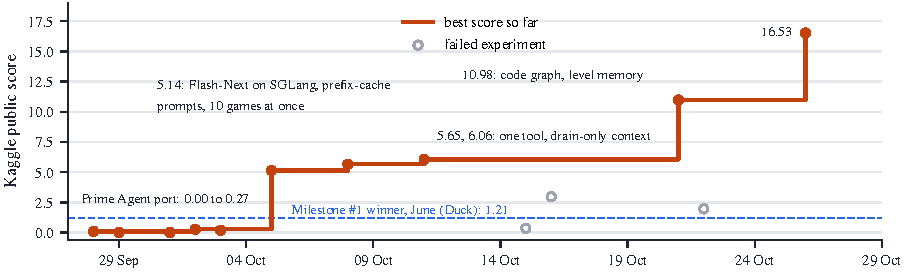
\includegraphics[width=\textwidth]{figures/leaderboard.pdf}
\caption{Every completed submission of our team to the Kaggle ARC-AGI-3 leaderboard (hidden games), with the main
change in each build. Hollow points are experiments that made things worse. They are kept on the plot, and each one
was rolled back. Four further submissions failed with Kaggle system errors during the rerun and have no score.}
\label{fig:leaderboard}
\end{figure*}

Figure~\ref{fig:leaderboard} shows the whole trajectory. The faithful port of Prime Agent's harness to open
weights scored 0.00--0.27. The model wrote code, but it brute-forced: in one 10-game run it reset 350 times and never
found a goal. Moving to Qwen3.8-Flash-Next on SGLang, with prompts laid out for the prefix cache and ten games at once,
took the score to 5.14. Merging the move tool into the Python tool and switching to drain-only context gave 5.65 and
6.06. The code graph, memory keyed by level and the one-request turn cycle gave 10.98. The current build, with
Duck-style draining and the briefing map switched back on, scored \textbf{16.53} on 26 October. That is 24 days after
0.27, and 13.7$\times$ the 1.21 that won Milestone~\#1 in June.

The field did not stand still. On the day we submitted, the leading entry scored 71.48, Tufa Labs' own current entry
68.91, and the 200th entry 32.69. In absolute terms \textsc{Sarbloh} is not competitive with these teams, and we do not
claim it is. What we claim is narrower: the curve, the engineering that produced it, and the parts of it that transfer.

\subsection{Same server, same model: against the Duck harness}

\begin{figure}[t]
\centering
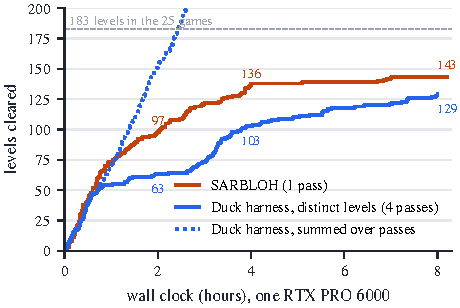
\includegraphics[width=\columnwidth]{figures/levels_vs_time.pdf}
\caption{Levels cleared over wall-clock time on the 25 public games, both agents on the same SGLang server and the
same Flash-Next weights. The Duck harness ran four passes of every game at once (100 runs). Solid blue counts a level
once per game, dotted blue counts it every time a pass clears it.}
\label{fig:curves}
\end{figure}

To separate the agent from the hardware, we ran a later release of the Tufa Labs Duck harness than the June winner on
\emph{our} server, with identical SGLang arguments and the same model. It played four passes of each public game
concurrently. Figure~\ref{fig:curves} compares it with our best single-pass run. \textsc{Sarbloh} clears 73 levels in
the first hour against 54, 97 against 63 at two hours, 136 against 103 at four, and 143 against 129 at 8.2 hours (of
183). Per GPU-hour the two agents are roughly equal: one Duck pass, which held about a quarter of the GPU, reached
about 104 levels. Our advantage is that the scheduler spends the same GPU on the games most likely to score next
rather than on four copies of each, so distinct levels arrive earlier. That matters under a hard nine-hour limit.

Figure~\ref{fig:pergame} breaks this down by game. With one pass against the Duck's best of four, \textsc{Sarbloh}
clears more levels in eight games, the largest gaps being \code{sk48} (8 against 0), \code{lf52} (6 against 1),
\code{wa30} (7 against 2) and \code{g50t} (6 against 3). The Duck does better in four (\code{tn36}, \code{vc33},
\code{s5i5}, \code{sp80}), and thirteen are tied. Both agents stall in \code{bp35}.

\begin{figure*}[t]
\centering
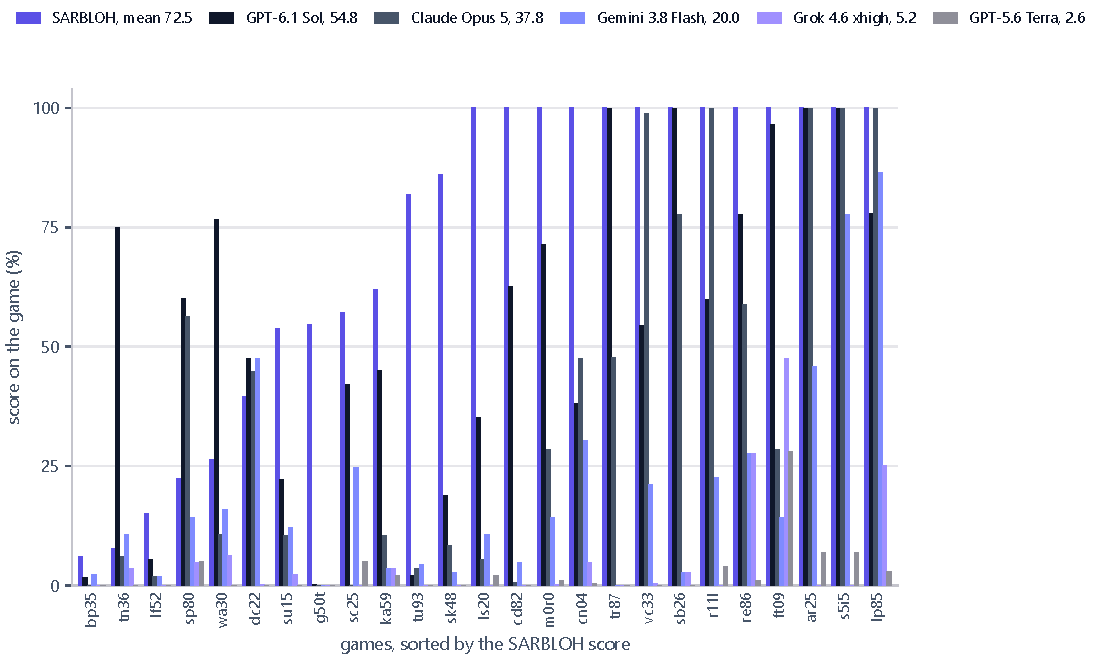
\includegraphics[width=\textwidth]{figures/per_game.pdf}
\caption{Levels cleared per public game: our single pass against the Duck harness's best of four passes, on the same
server. Games are sorted by our completion rate.}
\label{fig:pergame}
\end{figure*}

\subsection{Efficiency once a level is understood}

RHAE punishes every action quadratically, so we also measure how efficient the agent is on the levels it clears.
In the best run the \emph{median} cleared level took 0.77 of the human baseline's actions, which earns the 1.15 cap
(Eq.~\ref{eq:rhae}). Once the agent understands a level it plays it at or above human efficiency: it reasons in code
and sends the path. Taking the run's 59.4 mean public-game score as a reference (a development number on
contaminated games), the 40.6 points it lost split roughly into 12.6 from extra actions on cleared levels, 8.0 from 13
levels attempted but not solved, and 19.5 from levels never reached because a game stalled earlier. Most of the loss is
not inefficiency. It is levels the agent never came to understand.

\subsection{Where the GPU time goes}

\begin{table}[t]
\centering
\small
\begin{tabular}{@{}lr@{}}
\toprule
Measure (9-hour run, 25 games, one GPU) & Value \\
\midrule
Prompt tokens served from the prefix cache & \textbf{98.4\%} \\
Prompt tokens / reply tokens & 1.78\,B / 14.4\,M \\
Model calls / LLM failures & 21,224 / 0 \\
Games inside a turn at once (mean) & 11.8 \\
Turns per minute, all games & 42.7 \\
Decode speed per request & 76 tok/s \\
Turn wall time, median / p90 & 2.3\,s / 30.2\,s \\
Busy time decoding / prefilling & 50.1\% / 1.3\% \\
Share of reply text that is thinking & 78\% \\
Minutes per cleared level (median) & 9.2 \\
Actions / human baseline, cleared levels (median) & 0.77 \\
\bottomrule
\end{tabular}
\caption{Telemetry of the best offline run (143/183 levels), from the harness's own speed report.}
\label{tab:telemetry}
\end{table}

Table~\ref{tab:telemetry} shows that the system is decode-bound, which is what we designed for. Prefill takes 1.3\%
of busy time because 98.4\% of all prompt tokens are reused from the cache. Before the append-only rewrite, the same
agent reused about 10\% and prefill starved every other game. The server made 21,224 calls with no failures in nine
hours.

\subsection{What the numbers do not show}

\paragraph{The briefing has not been isolated.} The 143-level run sent the lettered board and the plain picture, with
the briefing and the map switched off. The 16.53 build had both switched on. Other changes landed between those builds,
so neither number measures the briefing alone. What the briefing does have is the lab evidence (\S\ref{sec:lab}) and
the oracle result (\S\ref{sec:motivation}). A same-model A/B on the hidden set is the next experiment.

\paragraph{Failure modes.} Thirteen levels were attempted and never solved. \code{bp35} and \code{sp80} stopped at level
2 in every full run we made. In the best run, four games came 2--15 moves short of the 2,000-action cap and the model
then answered ``\code{Holding...}'' to the continue prompt about 14,000 times, which burned 1.24\,B of the 1.78\,B
prompt tokens on turns that did nothing. The current build caps each game at 400 turns, which bounds such a stall. Finally, a negative result:
replacing old code in the history with a one-line stub, to save tokens, made the model write the stub \emph{as its
code} in 97.7\% of its calls, and the run cleared no level. A small model copies what it sees.

\section{Conclusion}
\label{sec:conclusion}

On an interactive benchmark scored by action efficiency, an agent cannot afford to reason its way around a bad view of
the world. Every probing move costs it quadratically. Our first experiments showed that for language models the view
is the first thing that fails: integers are nearly unreadable, a picture fixes most of it, and a few lines of meaning
fix much of the rest. \textsc{Sarbloh}'s perception engine supplies those lines from code. It states what geometry
proves, guesses what it cannot prove, and attaches to every guess the single action that would settle it. The perception
lab showed why that split matters: single-frame guesses were right about half the time on games they were not designed
on, so they have to be labelled as guesses.

Around the engine, the rest is engineering for a fixed GPU budget. The agent acts in code and sends whole paths. The
prompt only grows, so 98.4\% of it stays cached. A scheduler hands the GPU to whichever game is most likely to score
next. With these pieces a 6B-active open model clears 143 of 183 public levels in one pass, matches a strong harness
per GPU-hour while reaching more distinct levels in the same time, and took our hidden-set score from 0.27 to 16.53 in
24 days.

\paragraph{Limitations.} The briefing's own contribution on the hidden set has not been isolated by a same-model A/B.
The Gemini ladder and the oracle briefing are single runs that motivate the design; they do not measure it. Public-game
numbers are contaminated. Our absolute score is far below the leading entries, and much of what remains lost is levels
the agent never comes to understand, which is the problem this paper argues perception should attack next.

\paragraph{Next.} A clean briefing A/B on the hidden set, perception that updates its role guesses from the outcomes of
their tests, and LoRA fine-tuning \citep{hu2021lora} on our own cleared-level traces, with GRPO \citep{shao2024grpo}
tried only if it beats supervised fine-tuning within the same GPU budget. Both pipelines are already built.


\bibliography{references}

\clearpage
\appendix
\sloppy
\section{The briefings of Figure~\ref{fig:views}}
\label{app:briefings}

This is the engine's output, copied without edits, for the first frames shown in Figure~\ref{fig:views} (the
20-line cap, as the agent sees it). The object ids match the map.

\paragraph{\code{ls20} (arrow keys).}
\begin{lstlisting}
BRIEFING (arrow keys)
MEASURED (certain):
- Floor is a 5x5 tile grid.
- obj 4 (blue 6-cell shape): sits inside a black box that is NOT plain floor; the floor reaches the box's bottom side in 5 steps (the only way in)
- obj 6 (white/light grey plus): reachable in 6 steps
- obj 4 (blue 6-cell shape) is directly above obj 10 (blue/orange square) (shared columns 35-37)
- obj 12 (blue irregular shape (24 cells)) (drawn 2x bigger), mirrored left-right OR turned 90 deg clockwise, becomes exactly obj 4 (blue 6-cell shape)
- 3 identical red square (2x2): obj 16, 17, 18 -> a count of something (lives, items, tiles)
- obj 6 (white/light grey plus) has a symmetric shape but lopsided colours (marks a direction/state)
- obj 10 (blue/orange square) has a symmetric shape but lopsided colours (marks a direction/state)
GUESSES (check with one action):
- obj 10 (blue/orange square) = YOU (80%) - test: press one arrow key: it should move one tile and the gauge should drop
- obj 12 (blue irregular shape (24 cells)) = INVENTORY (80%) - test: watch it after touching the modifier
- obj 4 (blue 6-cell shape) = GOAL (75%) - test: get the right thing into it and see if the level ends
- obj 15 (yellow bar) = MOVES LEFT (75%) - test: take any action and check it shrinks by one unit
- obj 16, 17, 18 (red square) = LIVES (75%) - test: watch it when the gauge runs out or you fail
- obj 6 (white/light grey plus) = MODIFIER (67%) - test: step onto it, then check whether the inventory icon changed
\end{lstlisting}

\paragraph{\code{r11l} (clicks).}
\begin{lstlisting}
BRIEFING (clicks)
MEASURED (certain):
- no tile grid -> free movement. Open space = black (81% of screen).
- all 4 main objects share one open space; straight paths between them are ALL CLEAR of rock
- the grey areas are not open floor (likely walls)
- obj 4 (purple dotted ring) encloses an EMPTY 5x5 space -- exactly the size of: obj 16 (white/purple diamond), obj 25 (purple/magenta disc), obj 36 (dark grey/purple diamond)
- a light grey line connects obj 16 (white/purple diamond) to obj 25 (purple/magenta disc)
- a light grey line connects obj 25 (purple/magenta disc) to obj 36 (dark grey/purple diamond)
- obj 25 (purple/magenta disc) sits at the MIDPOINT of obj 16 (white/purple diamond) and obj 36 (dark grey/purple diamond) (error 0.5 cells) -> it is held between them; moving either end should move it to the new midpoint
- obj 16, 36 (white/purple diamond; dark grey/purple diamond) have the same shape in different colours (white/purple vs dark grey/purple)
GUESSES (check with one action):
- obj 4 (purple dotted ring) = GOAL (80%) - test: get the right thing into it and see if the level ends
- obj 16, 36 (white/purple diamond; dark grey/purple diamond) = HANDLE (click) (80%) - test: click an empty spot once: the selected handle should jump there
- obj 1 (white bar) = MOVES LEFT (75%) - test: take any action and check it shrinks by one unit
- obj 25 (purple/magenta disc) = CARRIED THING (75%) - test: move one handle: it should slide to the new midpoint
\end{lstlisting}

\section{Configuration of the scored runs}
\label{app:config}

\begin{table}[h]
\centering
\footnotesize
\setlength{\tabcolsep}{3pt}
\begin{tabular}{@{}L{0.5\columnwidth}L{0.46\columnwidth}@{}}
\toprule
Knob & Value \\
\midrule
Games / GPU slots / scheduler quantum & 25 / 10 / 20 calls \\
Action budget per game & 2,000 \\
Moves per \code{play()} path & $\le$100 \\
Reply budget / inner requests per turn & 12k tokens / 12 \\
Thinking before a turn yields & 16k tokens \\
Drain trigger / target / window & 118k / 55k / 131k tokens \\
Reasoning effort & \code{xhigh} \\
Picture & 10 px per cell, newest only, stored once \\
Briefing / short-view caps & 20 lines / 600 tokens \\
Memory caps (goal/plan/hyp./find.) & 150/200/400/300 tokens \\
Sampling & $T{=}0.6$, top-$p$ 0.95, top-$k$ 20 \\
Server & SGLang, W4A16, EAGLE 3 steps, FP8 KV \\
\bottomrule
\end{tabular}
\caption{Main settings (from \code{harness/config.py} and the notebook overrides).}
\end{table}

\section{Reproducing the figures}
Every number in this paper is produced by four scripts in \code{Writing/scripts/}: \code{collect\_data.py} (the Kaggle
submission history, the per-game table and the lab scores, each with its source), \code{extract\_curves.py} (levels
over time from the run logs), \code{make\_perception\_figure.py} (renders real frames through the agent's own
\code{perception.py}), and \code{plot\_results.py}. The experiment log, with every hypothesis, kill criterion and
verdict, is in \code{experiments/}.


\end{document}
